% ЕМТ 2018, V клас — точен LaTeX препис от официалните файлове в Klasirane.com.
% Условия: https://klasirane.com/api/competitions/EMT/All/2018/5%20%D0%BA%D0%BB/probs
% SHA-256 (условия): 9cb7cdb78f726fcac5cbd32529373909e352d8ea1fc01ef29db3263367c386fb
% Решения: https://klasirane.com/api/competitions/EMT/All/2018/5%20%D0%BA%D0%BB/sol
% SHA-256 (решения): dd77262544cb5e06e6f2748e213b23800cb7eeb0151be68f78909349ecf8b729
% Точковите оценки, правописът и непълнотите са запазени от източника.

Задача 5.1. Иван установил, че през $n$-тата седмица на 2018 година ще останат точно $n^2$ дни до края на годината. Намерете $n$ и точно през кой ден от седмицата ще се случи тази закономерност?

Решение. Равенството, което удовлетворява условието е: $n^2=365-7(n-1)-d$. \hfill 5 т.

С $n$ сме означили номерът на седмицата, а с $d$ - ден от седмицата в който се е случило събитието. $d$ е число от 1 до 7.

Оттук получаваме $n^2+7n=372-d$ или $n(n+7)=372-d$.

След проверка при $d=1\ldots 7$ \hfill 4 т.

При $n=16$ имаме $16.23=368=372-4.d=4$ \hfill 1 т.

Отг. 16 седмица, четвъртък

Задача 5.2. Намерете такова естествено число $A$, че $2.A$ да е точна втора степен на естествено число, $3.A$ да е точна трета степен на естествено число и $5.A$ да е точна пета степен на естествено число.

Решение. $2.A=a.a$, $3.A=b.b.b$, $5.A=c.c.c.c.c$

В разлагането на числото $A$ трябва да има $k$ пъти множител 2, където $k$ е нечетно число. \hfill 1 т.

От второто и третото равенство $k$ трябва да е кратно на 3 и 5.

Следователно $k$ може да е $15,45\ldots$. \hfill 2 т.

В разлагането на числото $A$ трябва да има $s$ пъти множител 3, където $s+1$ се дели на 3. \hfill 1 т.

От първото и третото равенство $s$ трябва да е кратно на 2 и 5.

Следователно $s$ може да е $20,51\ldots$. \hfill 2 т.

В разлагането на числото $A$ трябва да има $p$ пъти множител 5, където $p+1$ се дели на 5. \hfill 1 т.

От първото и второто равенство $p$ трябва да е кратно на 2 и 3.

Следователно $p$ може да е $24,54\ldots$. \hfill 2 т.

За намиране на число от търсения вид. \hfill 1 т.

Отг. Най-малкото число $A$ с това свойство трябва да се дели на 15 двойки, на 20 тройки и на 24 петици.

Задача 5.3. На страните $BC$ и $CD$ на правоъгълника $ABCD$ са избрани съответно точки $M$ и $N$, като $BM=DN$. Ако правите $BN$ и $DM$ се пресичат в точка $P$, да се докаже точка $P$ е равни разстояния от страните $AB$ и $AD$.

Решение. За правилен чертеж. \hfill – 1 т.

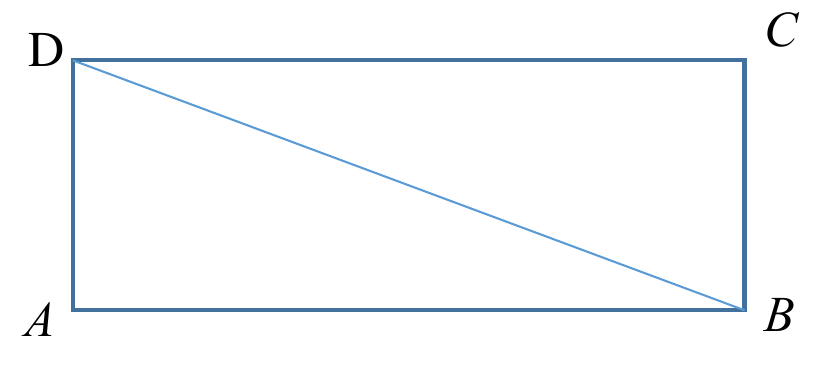
\includegraphics[max width=\textwidth, alt={Правоъгълник ABCD с диагонал DB}, center]{assets/5-3-solution-context.png}

Ще използваме, че диагоналът на правоъгълника го разделя на две части с равни лица (два равнолицеви триъгълника). Така $S_{ABCD}=2.S_{ABD}=2.S_{BCD}$. Така $(AB.AD):2=(CB.CD):2=S_{ABD}$. \hfill – 2 т.

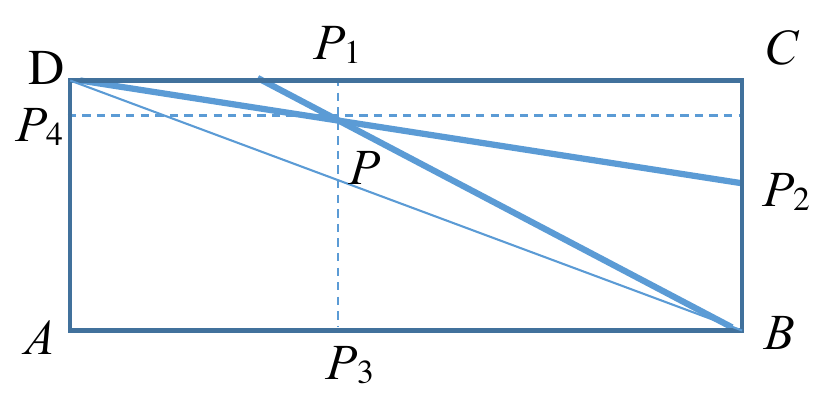
\includegraphics[max width=\textwidth, alt={Разделяне на правоъгълника през P с точки P1, P2, P3 и P4}, center]{assets/5-3-solution-proof.png}

Ще означим лицето на една триъгълна част, например $ABC$ с $[ABC]$. През точка $P$ разделяме правоъгълника на четири малки правоъгълника и нека $PP_1$ и $PP_2$ са разстоянията от точката $P$ съответно до страните $CD$ и $AB$. Ще покажем, че $PP_3=PP_4$. Чрез допълване до правоъгълник и изразяване на разлики на лица получаваме

$$[BDN]-[PDN]=[PDB]=[DBM]-[PBM].$$ \hfill – 3 т.

Да опишем лицата в горното равенство със отсечки

$$DN.AD-DN.PP_1=BM.AB-BM.PP_2.$$ \hfill – 3 т.

По условие $DN=BM$. Делим двете страни на $DN$ и получаваме:

$$AD-PP_1=AB-PP_2,$$ което трябваше да докажем. \hfill – 2 т.

Задача 5.4. В отбора по ръгби има 26 състезатели с номера $\{1,2,3,\ldots,25,26\}$. Треньорът отделил шест състезатели с номера $\{a_1,a_2,\ldots,a_6\}$, които няма да играят в следващия мач. Намерете номерата на състезателите $A\{a_1,a_2,\ldots,a_6\}$, ако знаете, че всички суми по двойки: $a_1+a_2$, $a_1+a_3$, $a_1+a_4$, $a_1+a_5$, $a_1+a_6$, $\ldots$, всички суми по тройки: $a_1+a_2+a_3$, $a_1+a_2+a_4$, $\ldots$, $a_4+a_5+a_6$, всички суми по четворки: $a_1+a_2+a_3+a_4$, $\ldots$, $a_2+a_3+a_4+a_5$ и всички суми по петици: $a_1+a_2+a_3+a_4+a_5$, $a_1+a_2+a_3+a_4+a_6$, $\ldots$, $a_2+a_3+a_4+a_5+a_6$ са различни числа (множеството $A$ от естествени числа с посоченото свойство наричаме е разпръснато множество) Докажете, че треньорът не може да определи седем състезатели от отбора, които с номерата си $B=\{b_1,b_2,\ldots,b_7\}$, за които да образуват разпръснато множество.

Решение. Допускаме, че можем да намерим седем естествени числа $B=\{b_1,b_2,\ldots,b_7\}$ и множеството е разпръснато. В множеството $B$ има 7 подмножества с един елемент, 21 подмножества с 2 елемента, 35 подмножества с 3 елемента и 35 подмножества с 4 елемента или общо $35+35+21+7=98$ подмножества, които имат 98 различни суми. (по 1 точка за всяко подмножество) \hfill 4 т.

От друго страна най-голямата възможна сума от 4 елемента на даденото множество е $23+24+25+26=98$, (2 т.) но тези четири числа не могат да участват в множеството $B$, защото $23+26=24+25$. Следователно най-голямата сума от 4 числа от даденото множество е 97, (2 т.) т.е. няма как 98 подмножества да получат 98 различни числа за суми. Противоречие. (2 т.)
